\PassOptionsToPackage{table}{xcolor}

\documentclass[
%	handout,
	notes=none,
	aspectratio=169
]{beamer}

% Comment out the following line to hide the notes
%\setbeameroption{show notes}

% Imports
\usepackage{listings}
\usepackage{amsfonts}
\usepackage{amsmath}
\usepackage{pythonhighlight}
\usepackage{pgfpages}
\usepackage{tabularx}
\usepackage{ifxetex,ifluatex}
\usepackage{etoolbox}
\usepackage{framed}

\mode<handout>{%
	\pgfpagesuselayout{8 on 1}[a4paper,border shrink=5mm]
	\setbeameroption{show notes}
}

% Graphics configuration
\graphicspath{{./graphics/}}
\DeclareGraphicsExtensions{.pdf,.jpeg,.png,.jpg,.pdf}

% Useful macros
\def\etal{{\it et al.}}
\def\etc{{\it etc.}}
\def\eg{{\it e.g.}}
\def\ie{{\it i.e.}}
\def\cf{{\it cf.}}
\def\qv{{\it q.v.}}
\def\qqv{{\it qq.v.}}
\def\st{s.t.\ }
\def\code{\tt}
\def\setsep{:}
\def\concat{\mathbin{|}}

\renewcommand{\thefootnote}{\fnsymbol{footnote}}
\newcommand{\prescite}[1]{\footnote{\cite{#1}}}
\newcommand{\prestext}[1]{\footnotetext{\cite{#1}}}
\newcommand{\emaillink}[1]{\href{mailto:#1}{\nolinkurl{#1}}}

\setlength{\parskip}{0.5em}

% Tables

\newcolumntype{L}[1]{>{\raggedright\arraybackslash\tiny}p{#1}}

% Program listings
\definecolor{listingbaground}{rgb}{.9,.9,.9}

\lstset{
	language=C,
	backgroundcolor=\color{listingbaground},
	extendedchars=true,
	basicstyle=\fontsize{5pt}{6pt}\ttfamily,
	showstringspaces=false,
	showspaces=false,
	numbers=left,
	numberstyle=\fontsize{5pt}{6pt}\ttfamily\color{gray},
	numbersep=5pt,
	tabsize=2,
	breaklines=true,
	showtabs=false,
	captionpos=b,
	xleftmargin=5mm,
	escapeinside={££}{££},
	framexleftmargin=5mm
}

% https://tex.stackexchange.com/questions/89574/language-option-supported-in-listings
\lstdefinelanguage{JavaScript}{
	keywords={typeof, new, true, false, catch, function, return, null, catch, switch, var, if, in, while, do, else, case, break},
	keywordstyle=\color{blue}\bfseries,
	ndkeywords={class, export, boolean, throw, implements, import, this},
	ndkeywordstyle=\color{darkgray}\bfseries,
	identifierstyle=\color{black},
	sensitive=false,
	comment=[l]{//},
	morecomment=[s]{/*}{*/},
	commentstyle=\color{purple}\ttfamily,
	stringstyle=\color{red}\ttfamily,
	morestring=[b]',
	morestring=[b]"
}

\lstdefinelanguage{QML}{
	keywords={typeof, new, true, false, catch, function, return, null, catch, switch, var, if, in, while, do, else, case, break, id, property, bool, string, int, decimal, target},
	keywordstyle=\color{blue}\bfseries,
	ndkeywords={Page, Example, Timer, Column, PageHeader, TextSwitch, Label},
	ndkeywordstyle=\color{teal}\bfseries,
	identifierstyle=\color{black},
	sensitive=true,
	comment=[l]{//},
	morecomment=[s]{/*}{*/},
	commentstyle=\color{green}\ttfamily,
	stringstyle=\color{red}\ttfamily,
	morestring=[b]',
	morestring=[b]"
}

\lstdefinelanguage{cpp}{
	keywords={class, public, private, try, throw, catch, this, return, null, switch, if, while, do, else, case, break, for, bool, void, const},
	keywordstyle=\color{blue}\bfseries,
	ndkeywords={Q_OBJECT, Q_CLASSINFO, Q_PROPERTY, Q_SLOTS, Q_SIGNALS, signals, slots, READ, WRITE, NOTIFY},
	ndkeywordstyle=\color{teal}\bfseries,
	identifierstyle=\color{black},
	sensitive=false,
	comment=[l]{//},
	morecomment=[s]{/*}{*/},
	commentstyle=\color{purple}\ttfamily,
	stringstyle=\color{red}\ttfamily,
	morestring=[b]',
	morestring=[b]"
}

\lstdefinelanguage{sh2}{
	keywords={dbus, send, zypper, python3},
	keywordstyle=\color{blue}\bfseries,
	ndkeywords={session, type, print, reply, dest},
	ndkeywordstyle=\color{teal}\bfseries,
	identifierstyle=\color{black},
	sensitive=false,
	comment=[l]{\#},
	morecomment=[s]{/*}{*/},
	commentstyle=\color{purple}\ttfamily,
	stringstyle=\color{red}\ttfamily,
	morestring=[b]',
	morestring=[b]"
}

% To allow the theme files to be placed in a subdirectory
\makeatletter
	\def\beamer@calltheme#1#2#3{%
		\def\beamer@themelist{#2}
		\@for\beamer@themename:=\beamer@themelist\do
		{\usepackage[{#1}]{\beamer@themelocation/#3\beamer@themename}}}

	\def\usefolder#1{
		\def\beamer@themelocation{#1}
	}
	\def\beamer@themelocation{}

% Quotation styling
% conditional for xetex or luatex
\newif\ifxetexorluatex
\ifxetex
  \xetexorluatextrue
\else
  \ifluatex
    \xetexorluatextrue
  \else
    \xetexorluatexfalse
  \fi
\fi
%
\ifxetexorluatex%
  \usepackage{fontspec}
  \newfontfamily\quotefont[Ligatures=TeX]{Source Sans Pro} % selects Libertine as the quote font
\else
  \usepackage[utf8]{inputenc}
  \usepackage[T1]{fontenc}
  \newcommand*\quotefont{\fontfamily{Source Sans Pro}} % selects Libertine as the quote font
\fi

\newcommand*\quotesize{60} % if quote size changes, need a way to make shifts relative
% Make commands for the quotes
\newcommand*{\openquote}
   {\tikz[remember picture,overlay,xshift=-3ex,yshift=-2.5ex]
   \node (OQ) {\quotefont\fontsize{\quotesize}{\quotesize}\selectfont``};\kern0pt}

\newcommand*{\closequote}[1]
  {\tikz[remember picture,overlay,xshift=3ex,yshift={#1}]
   \node (CQ) {\quotefont\fontsize{\quotesize}{\quotesize}\selectfont''};}

% select a colour for the shading
\definecolor{shadecolor}{HTML}{ffffff}

\newcommand*\shadedauthorformat{\emph} % define format for the author argument

% Now a command to allow left, right and centre alignment of the author
\newcommand*\authoralign[1]{%
  \if#1l
    \def\authorfill{}\def\quotefill{\hfill}
  \else
    \if#1r
      \def\authorfill{\hfill}\def\quotefill{}
    \else
      \if#1c
        \gdef\authorfill{\hfill}\def\quotefill{\hfill}
      \else\typeout{Invalid option}
      \fi
    \fi
  \fi}
% wrap everything in its own environment which takes one argument (author) and one optional argument
% specifying the alignment [l, r or c]
%
\newenvironment{shadequote}[2][l]%
{\authoralign{#1}
\ifblank{#2}
   {\def\shadequoteauthor{}\def\yshift{-2ex}\def\quotefill{\hfill}}
   {\def\shadequoteauthor{\par\authorfill\shadedauthorformat{#2}}\def\yshift{2ex}}
\begin{snugshade}\begin{quote}\openquote}
{\shadequoteauthor\quotefill\closequote{\yshift}\end{quote}\end{snugshade}}




\usefolder{theme}
\usetheme{sailfish}

\begin{document}

\title{Daily blogging embedded Gecko development}
\subtitle{FOSDEM'24\\FOSS on Mobile Devroom}
\author{David Llewellyn-Jones}
\date{3rd February 2024}

%%%%%%%%%%%%%%%%%%%%%%%%%%%%%%%%%%%%%%%%%

\renewcommand{\thefootnote}{\arabic{footnote}}

\frame{
\titlepage
}
\note{
}

\renewcommand{\thefootnote}{\fnsymbol{footnote}}

%%%%%%%%%%%%%%%%%%%%%%%%%%%%%%%%%%%%%%%%%

\begin{frame}
\frametitle{About me}

\begin{columns}[T]
\begin{column}[T]{0.5\textwidth}
\setlength{\parskip}{0.5em}

\vspace{1.5cm}
\begin{enumerate}
\setlength{\parskip}{0.5em}
\item First
\item Second
\item Third
\end{enumerate}

\end{column}
\begin{column}[T]{0.5\textwidth}
\setlength{\parskip}{0.5em}

\vspace{1.5cm}
\begin{enumerate}
\setlength{\parskip}{0.5em}
\item First
\item Second
\item Third
\end{enumerate}

\end{column}
\end{columns}

\end{frame}
\note{
}

%%%%%%%%%%%%%%%%%%%%%%%%%%%%%%%%%%%%%%%%%

\begin{frame}
\frametitle{Linux on Mobile History}

\begin{columns}[T]
\begin{column}[T]{1.1\textwidth}

\vspace{0.5cm}
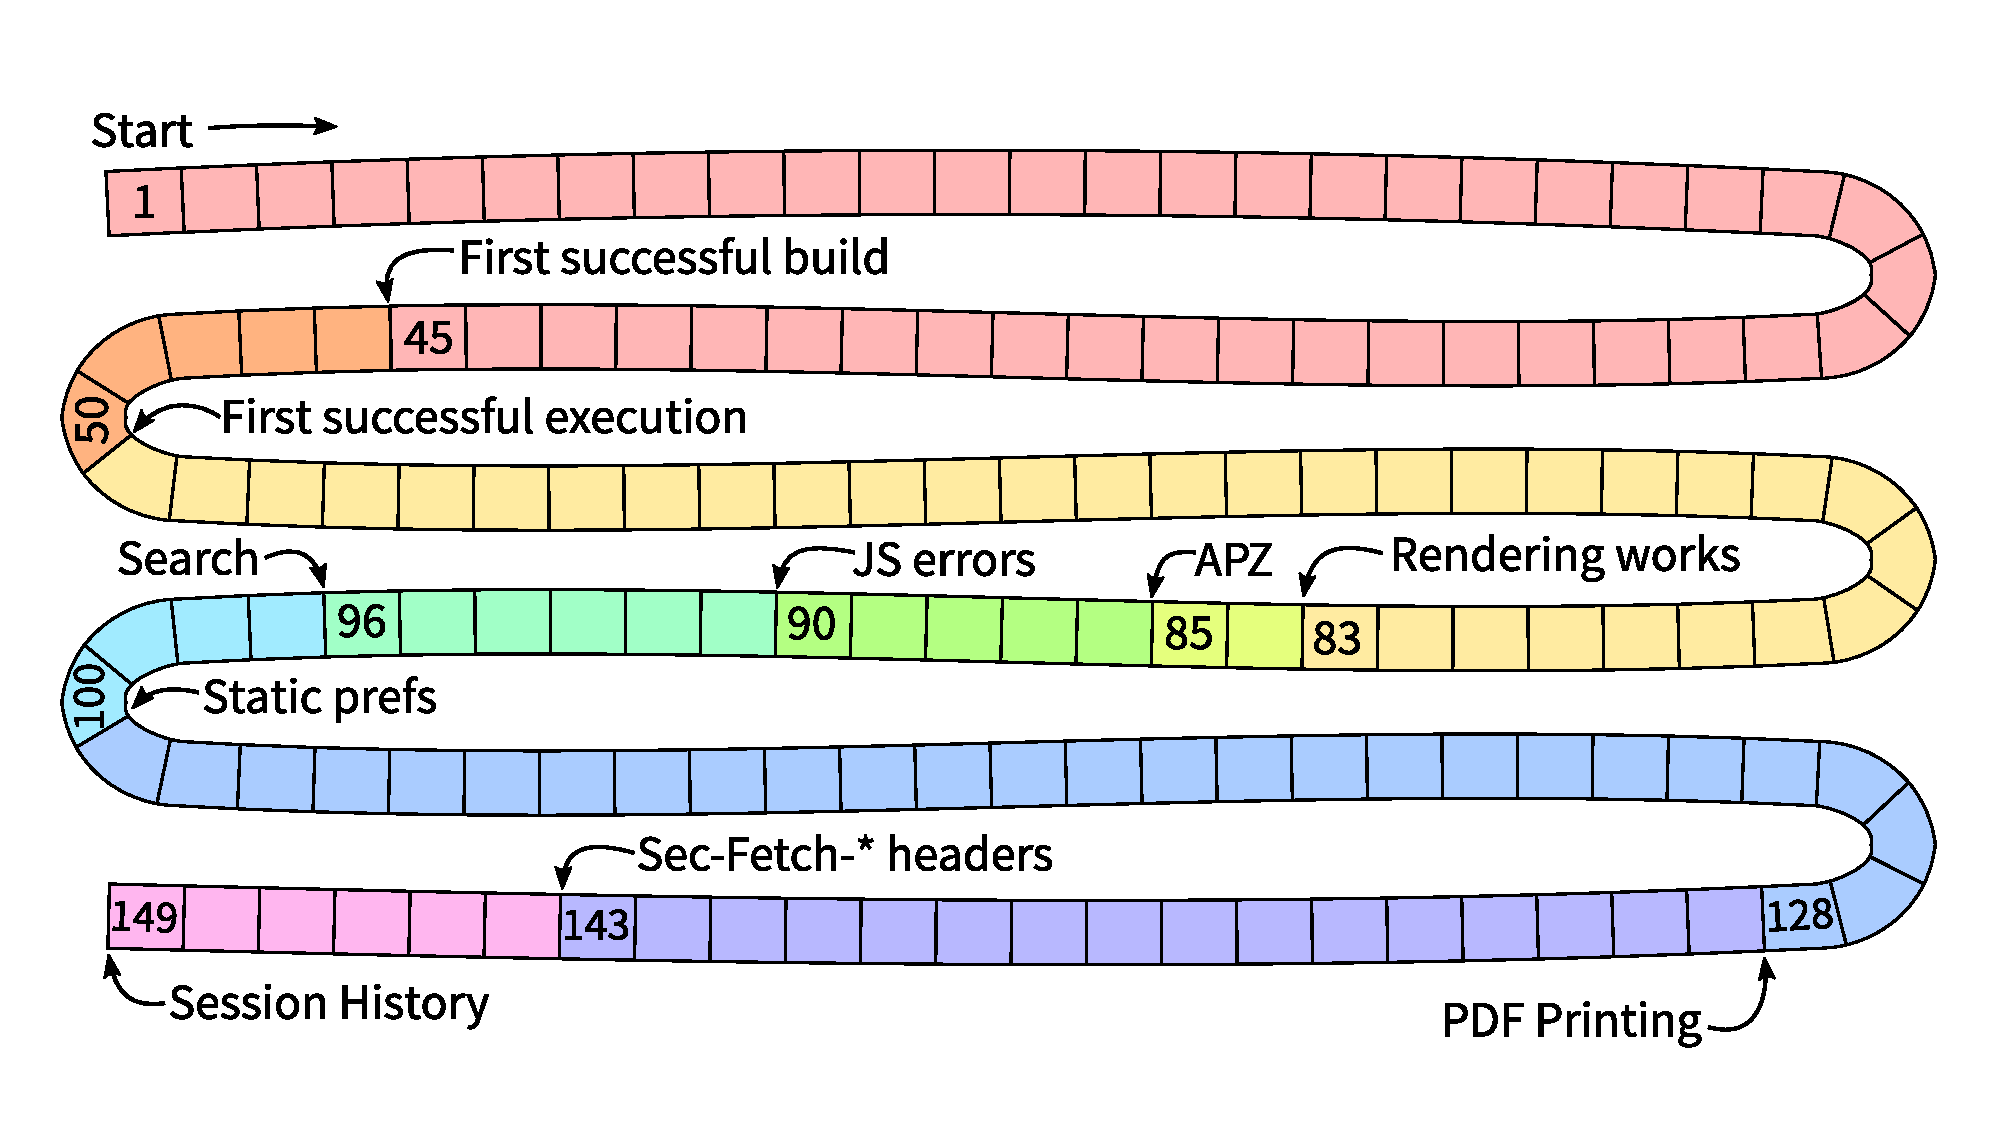
\includegraphics[width=1.0\textwidth]{timeline}

\end{column}
\end{columns}

\end{frame}
\note{
}

%%%%%%%%%%%%%%%%%%%%%%%%%%%%%%%%%%%%%%%%%

\begin{frame}
\frametitle{Maemo 4.1}

\begin{columns}[T]
\begin{column}[T]{1.0\textwidth}

\vspace{0.5cm}
\begin{center}
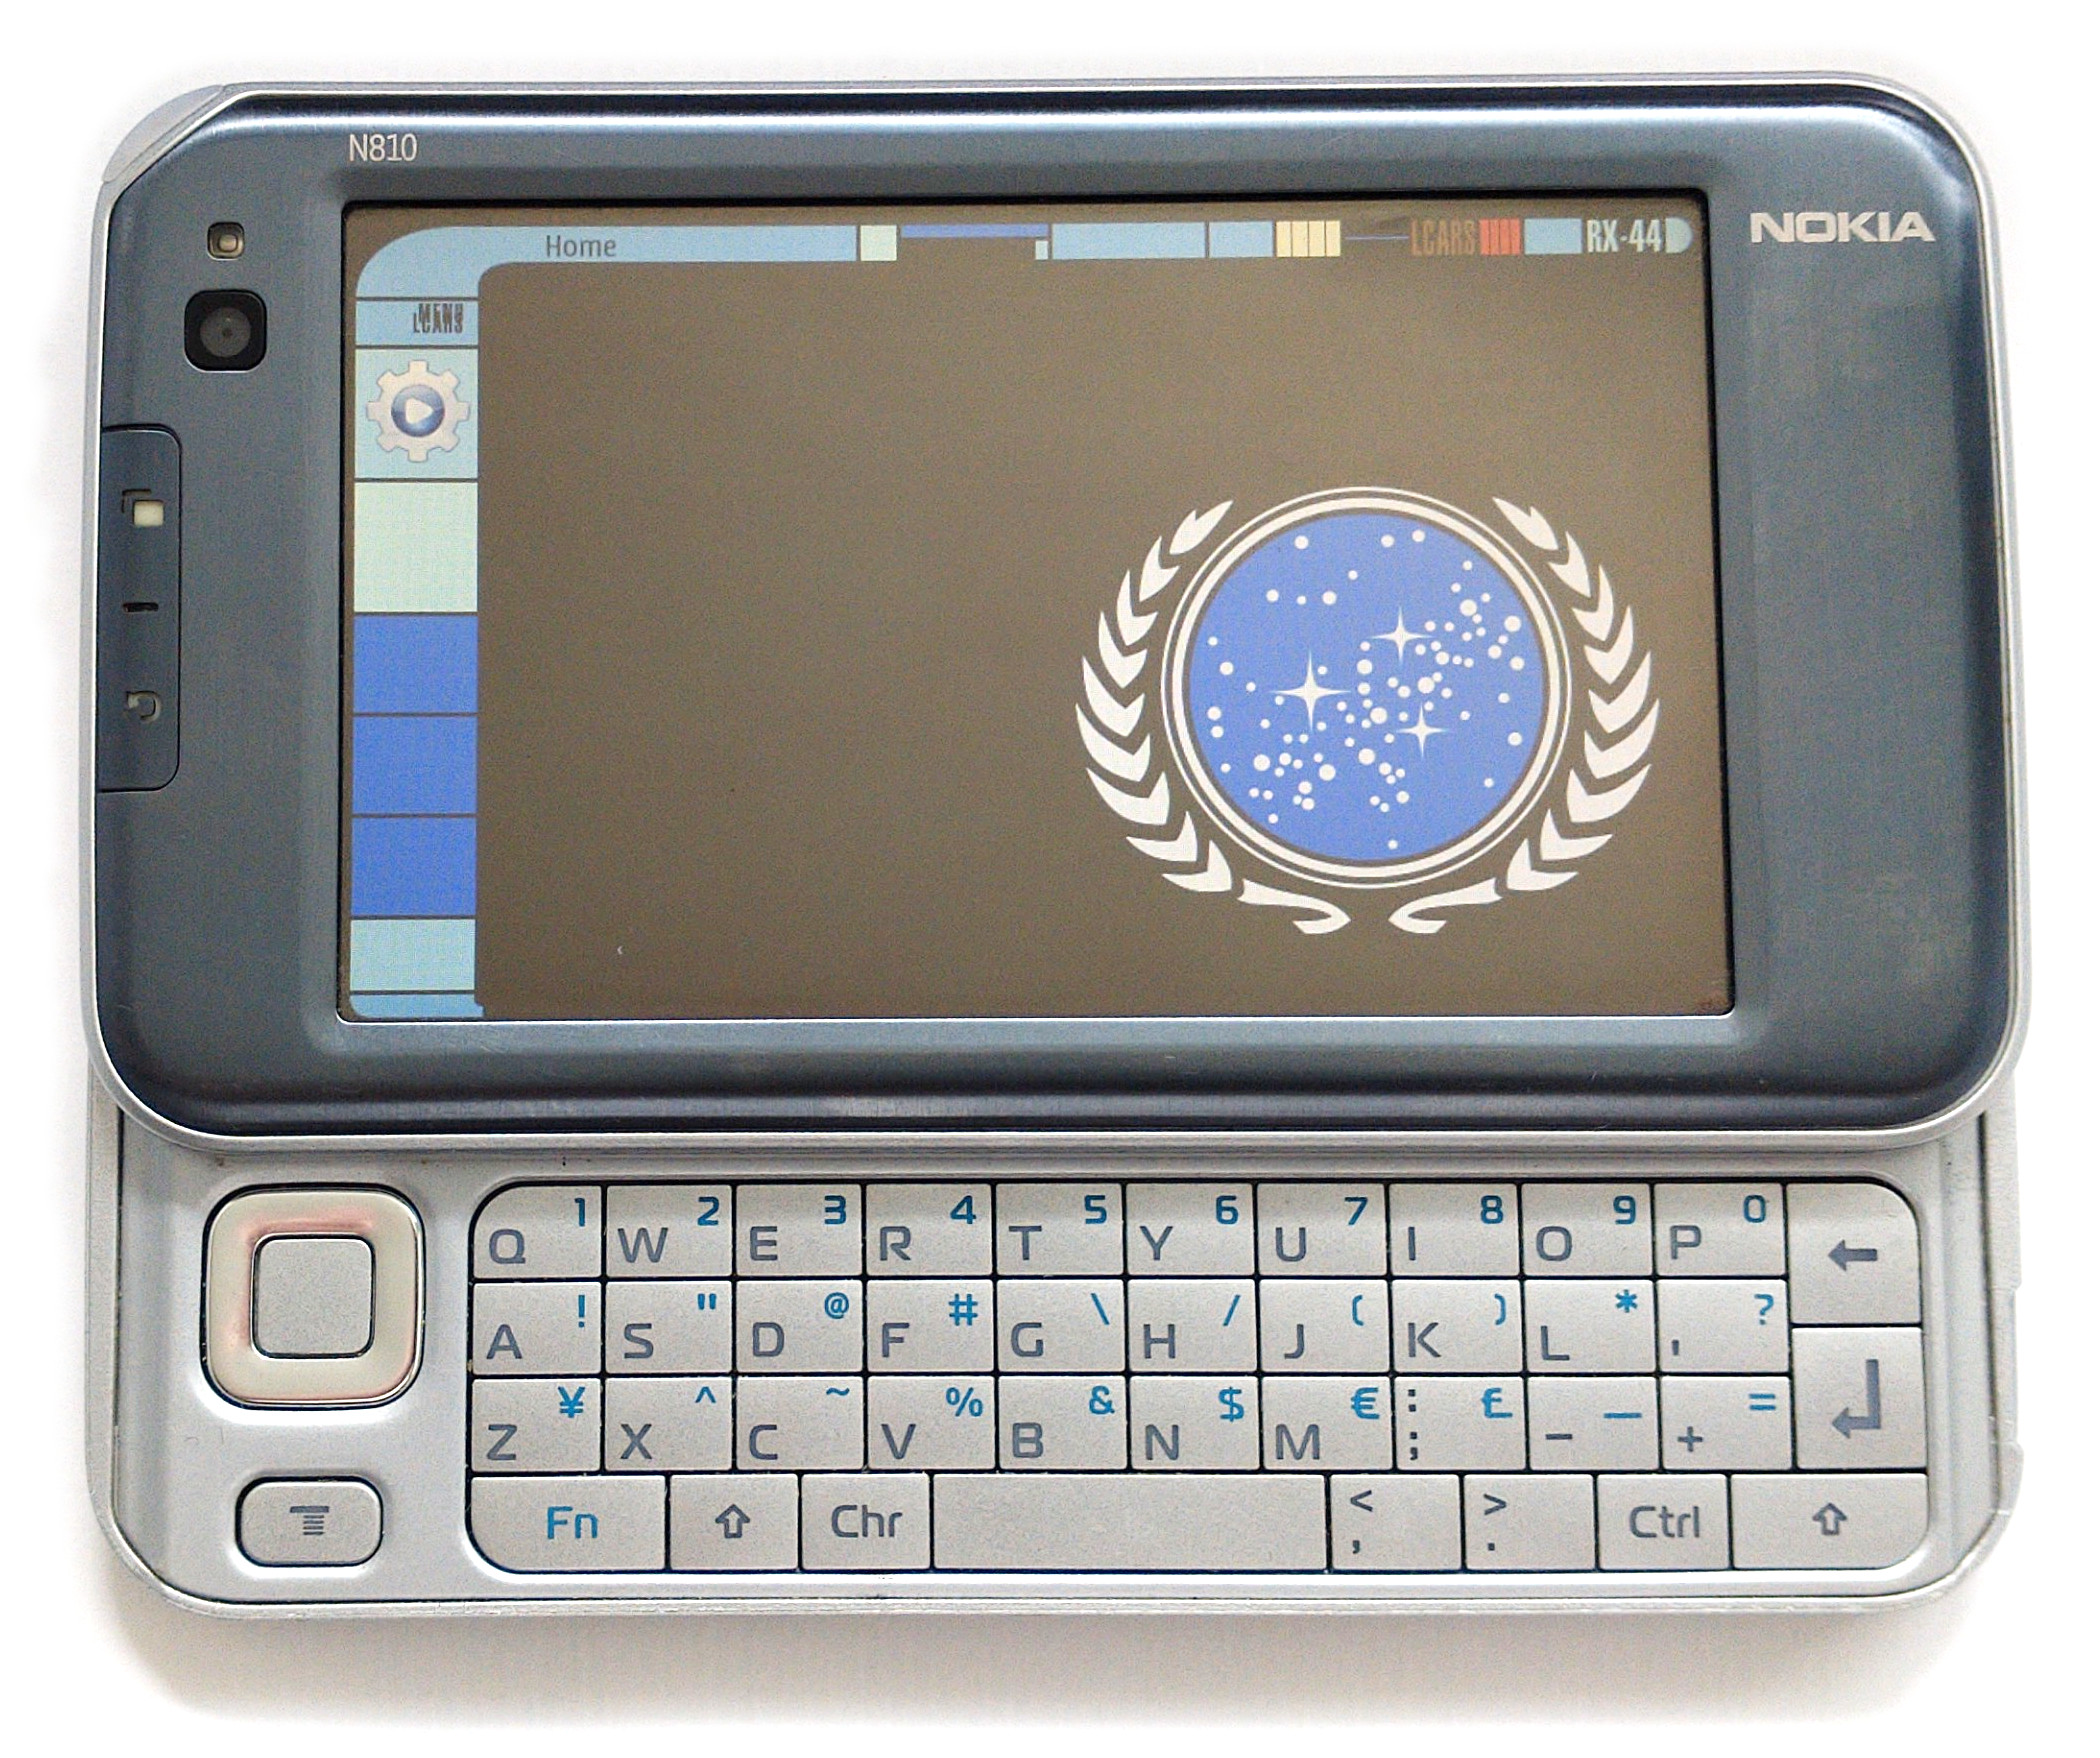
\includegraphics[width=0.6\textwidth]{n810}
\end{center}

\end{column}
\end{columns}

\end{frame}
\note{
}

%%%%%%%%%%%%%%%%%%%%%%%%%%%%%%%%%%%%%%%%%

\begin{frame}
\frametitle{Maemo 5}

\begin{columns}[T]
\begin{column}[T]{1.0\textwidth}

\vspace{0.8cm}
\begin{center}
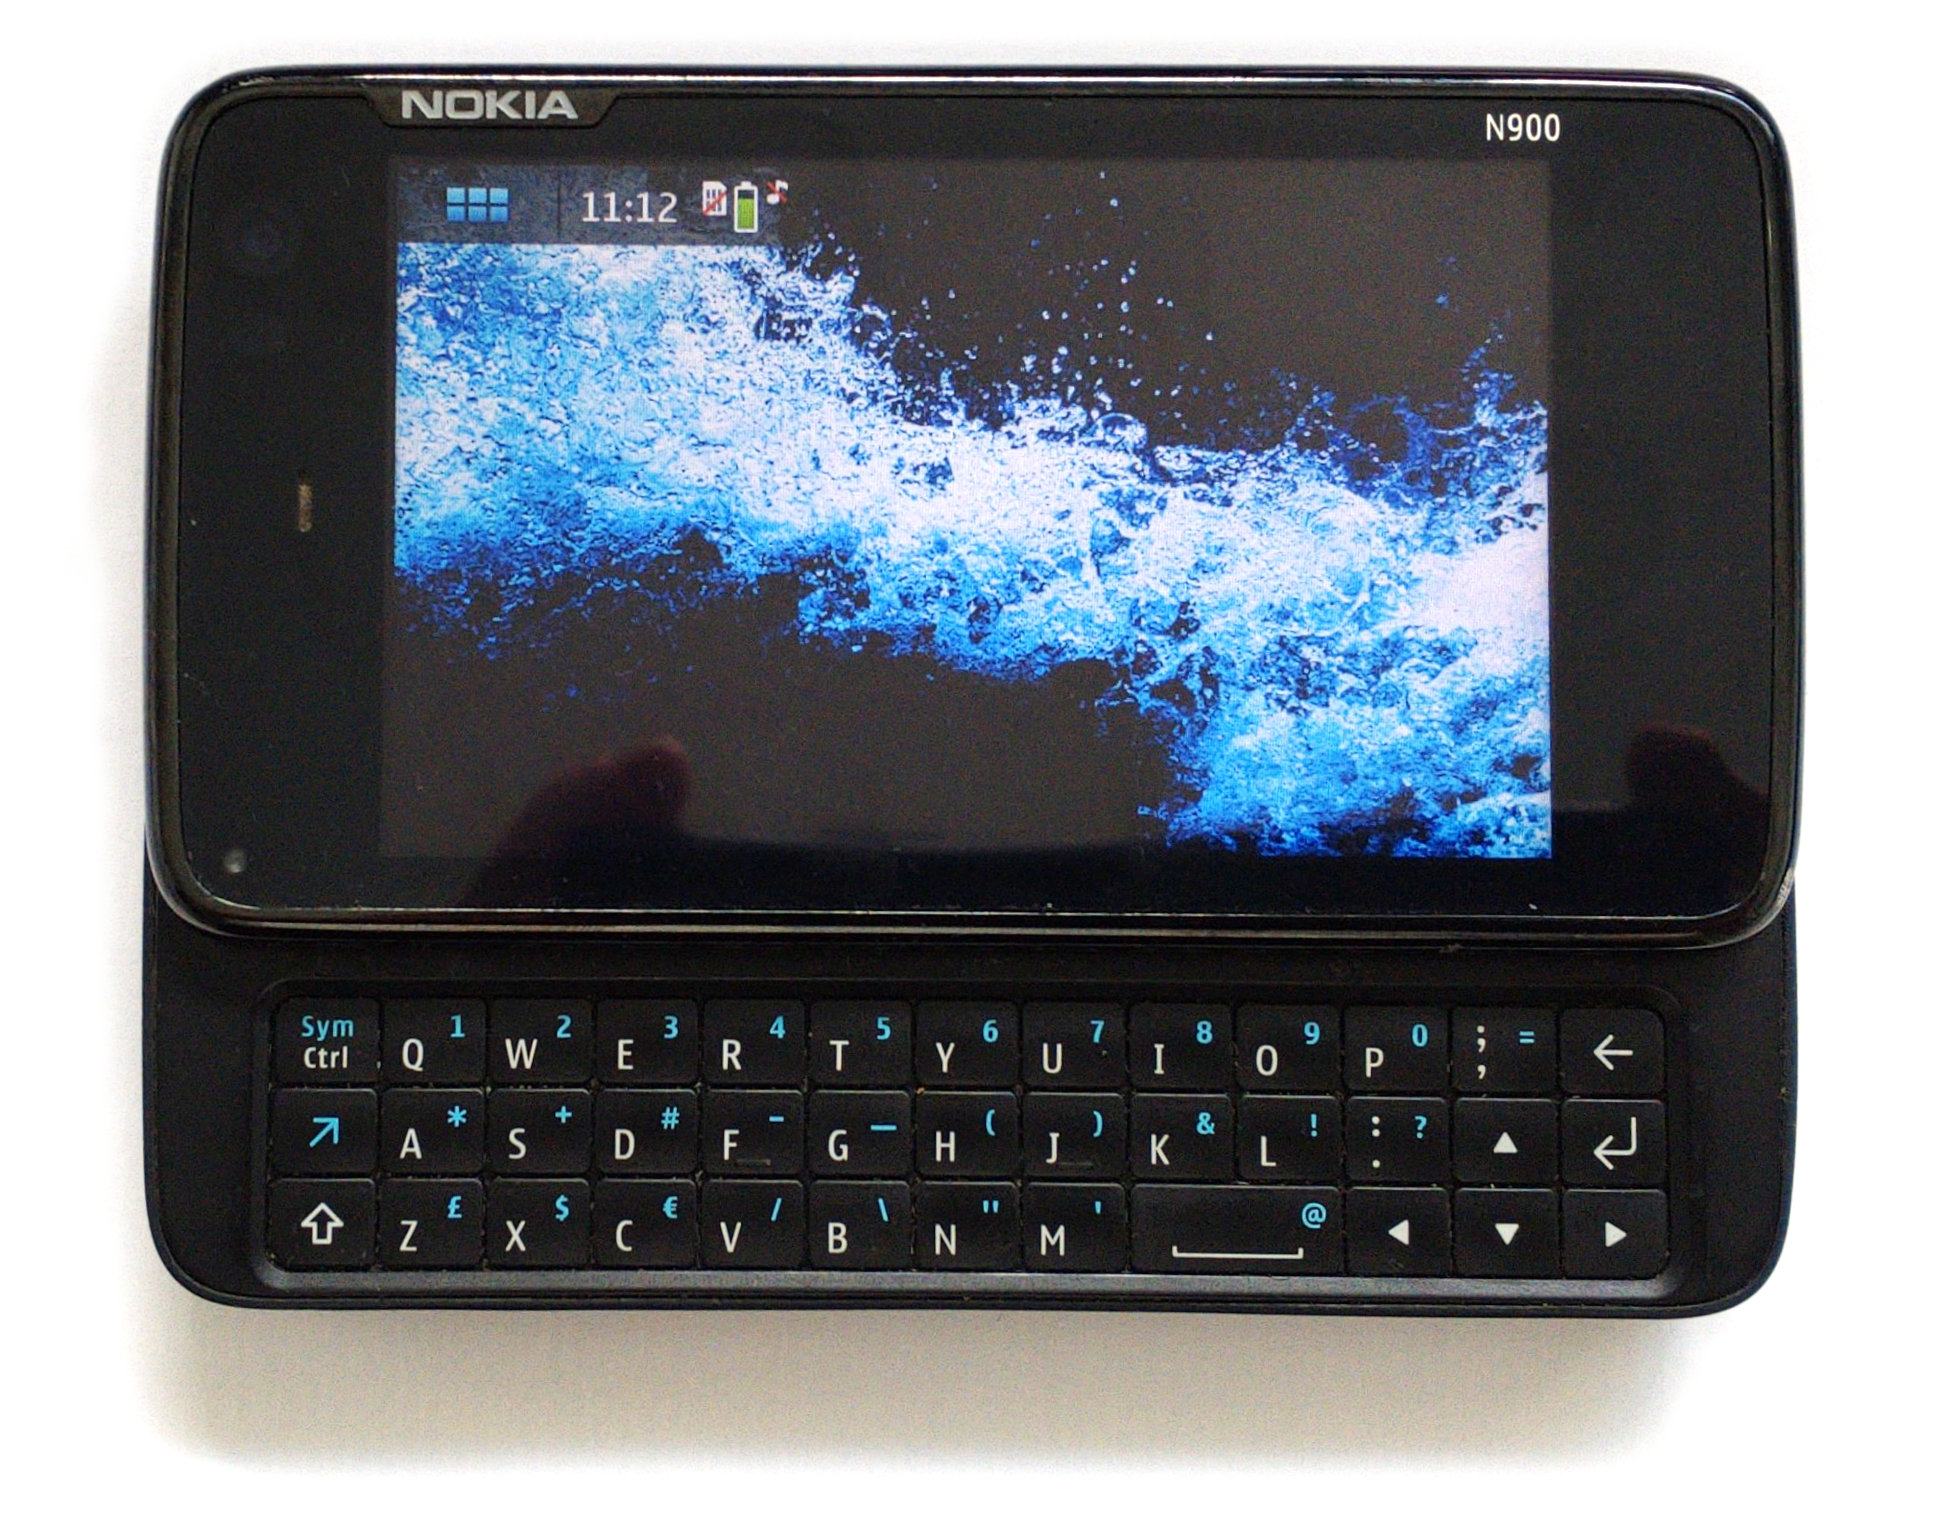
\includegraphics[width=0.6\textwidth]{n900}
\end{center}

\end{column}
\end{columns}

\end{frame}
\note{
}

%%%%%%%%%%%%%%%%%%%%%%%%%%%%%%%%%%%%%%%%

\begin{frame}
\frametitle{Sailfish OS 4.5}

\begin{columns}[T]
\begin{column}[T]{1.0\textwidth}

\vspace{0.3cm}
\begin{center}
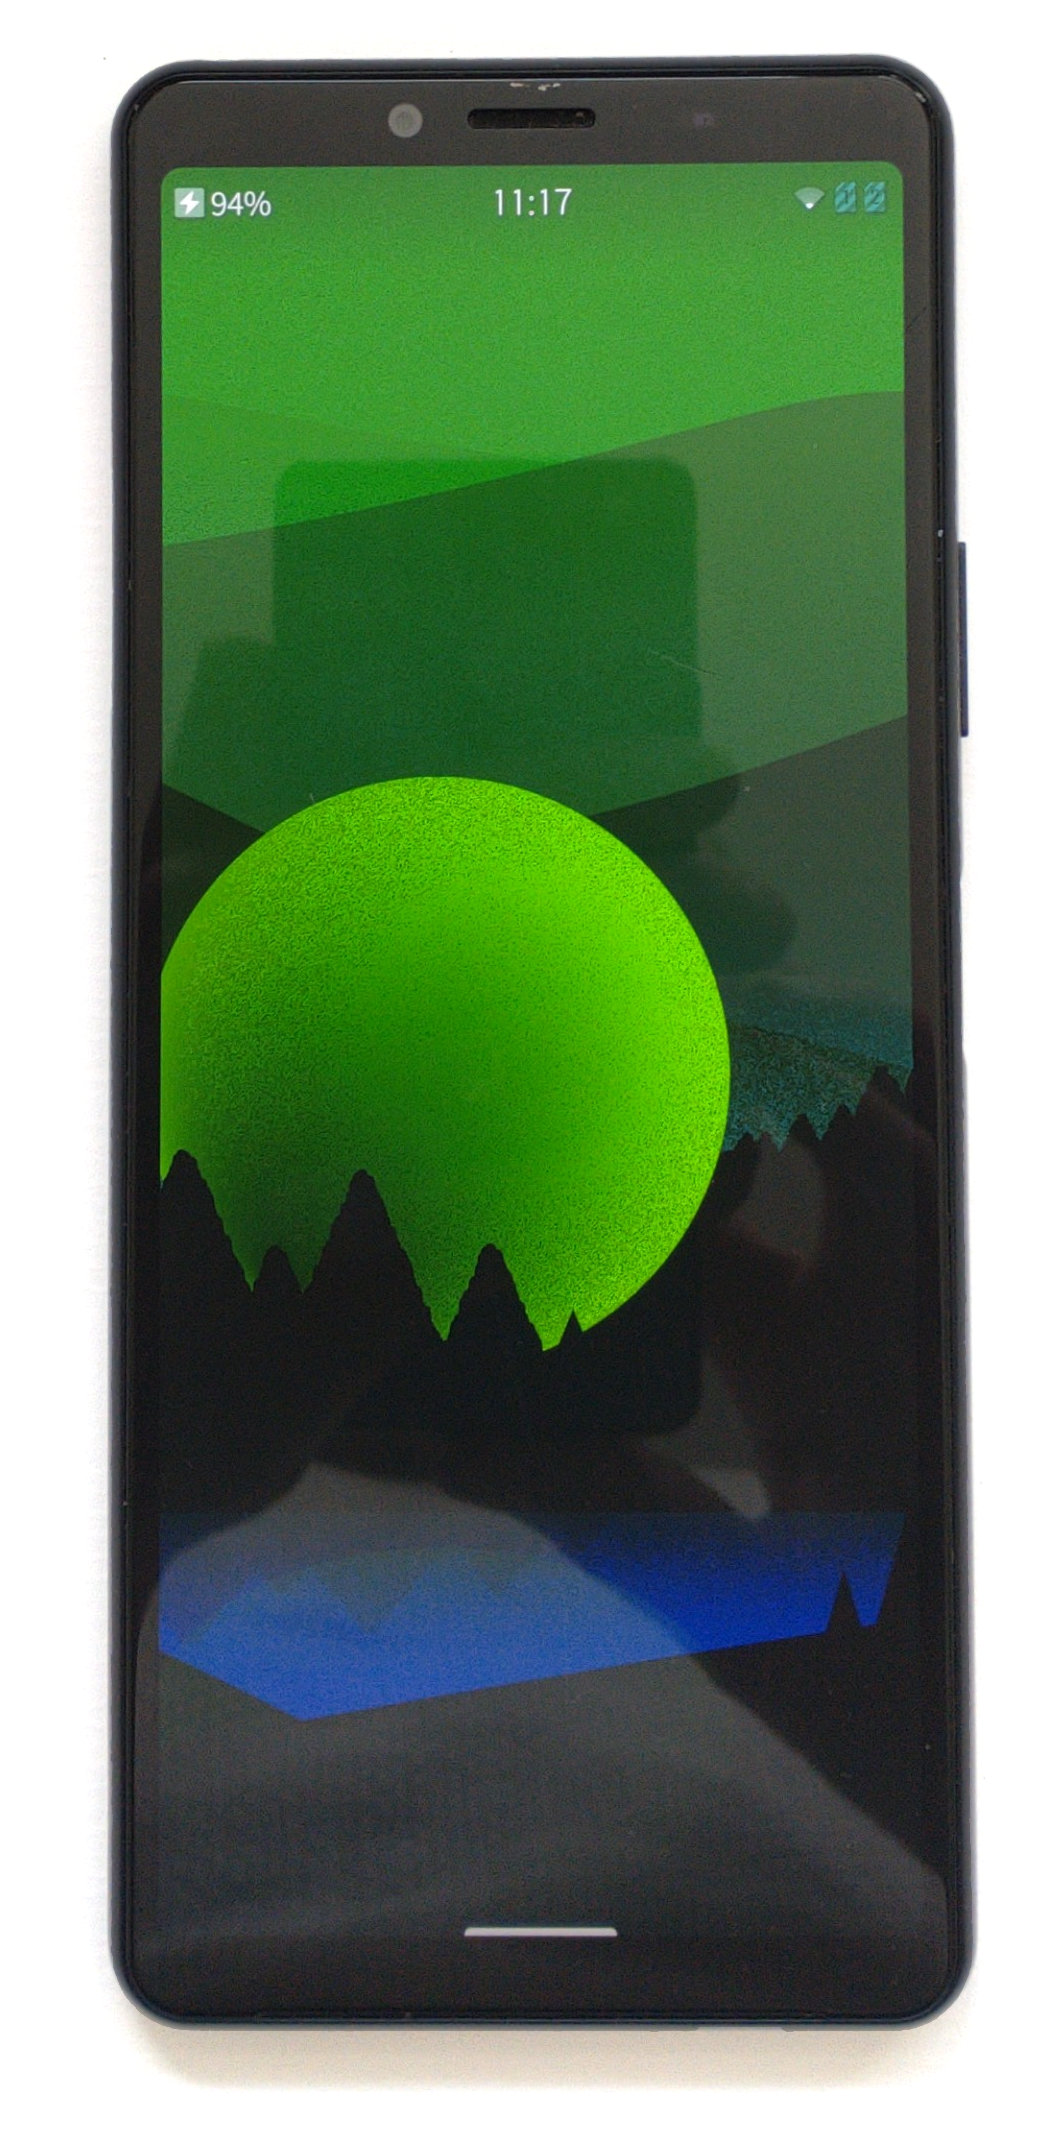
\includegraphics[width=0.26\textwidth]{xperia10ii}
\end{center}

\end{column}
\end{columns}

\end{frame}
\note{
}

%%%%%%%%%%%%%%%%%%%%%%%%%%%%%%%%%%%%%%%%%

\begin{frame}
\frametitle{Three Pillars of Sailfish OS}

\begin{columns}[T]
\begin{column}[T]{1.0\textwidth}

\vspace{0.5cm}
\begin{center}

\includegraphics[width=0.7\textwidth]{pillars}
\end{center}

\end{column}
\end{columns}

\end{frame}
\note{
}

%%%%%%%%%%%%%%%%%%%%%%%%%%%%%%%%%%%%%%%%%

\begin{frame}
\frametitle{Sailfish OS Stack}

\begin{columns}[T]
\begin{column}[T]{0.5\textwidth}
\setlength{\parskip}{0.5em}

\vspace{1.5cm}
\begin{enumerate}
\setlength{\parskip}{0.5em}
\item Android drivers
\item Libhybris and Libgbinder
\item Linux kernel 4.19.248
\item glibc
\item systemd
\item busybox
\end{enumerate}

\end{column}
\begin{column}[T]{0.5\textwidth}
\setlength{\parskip}{0.5em}

\vspace{0.0cm}
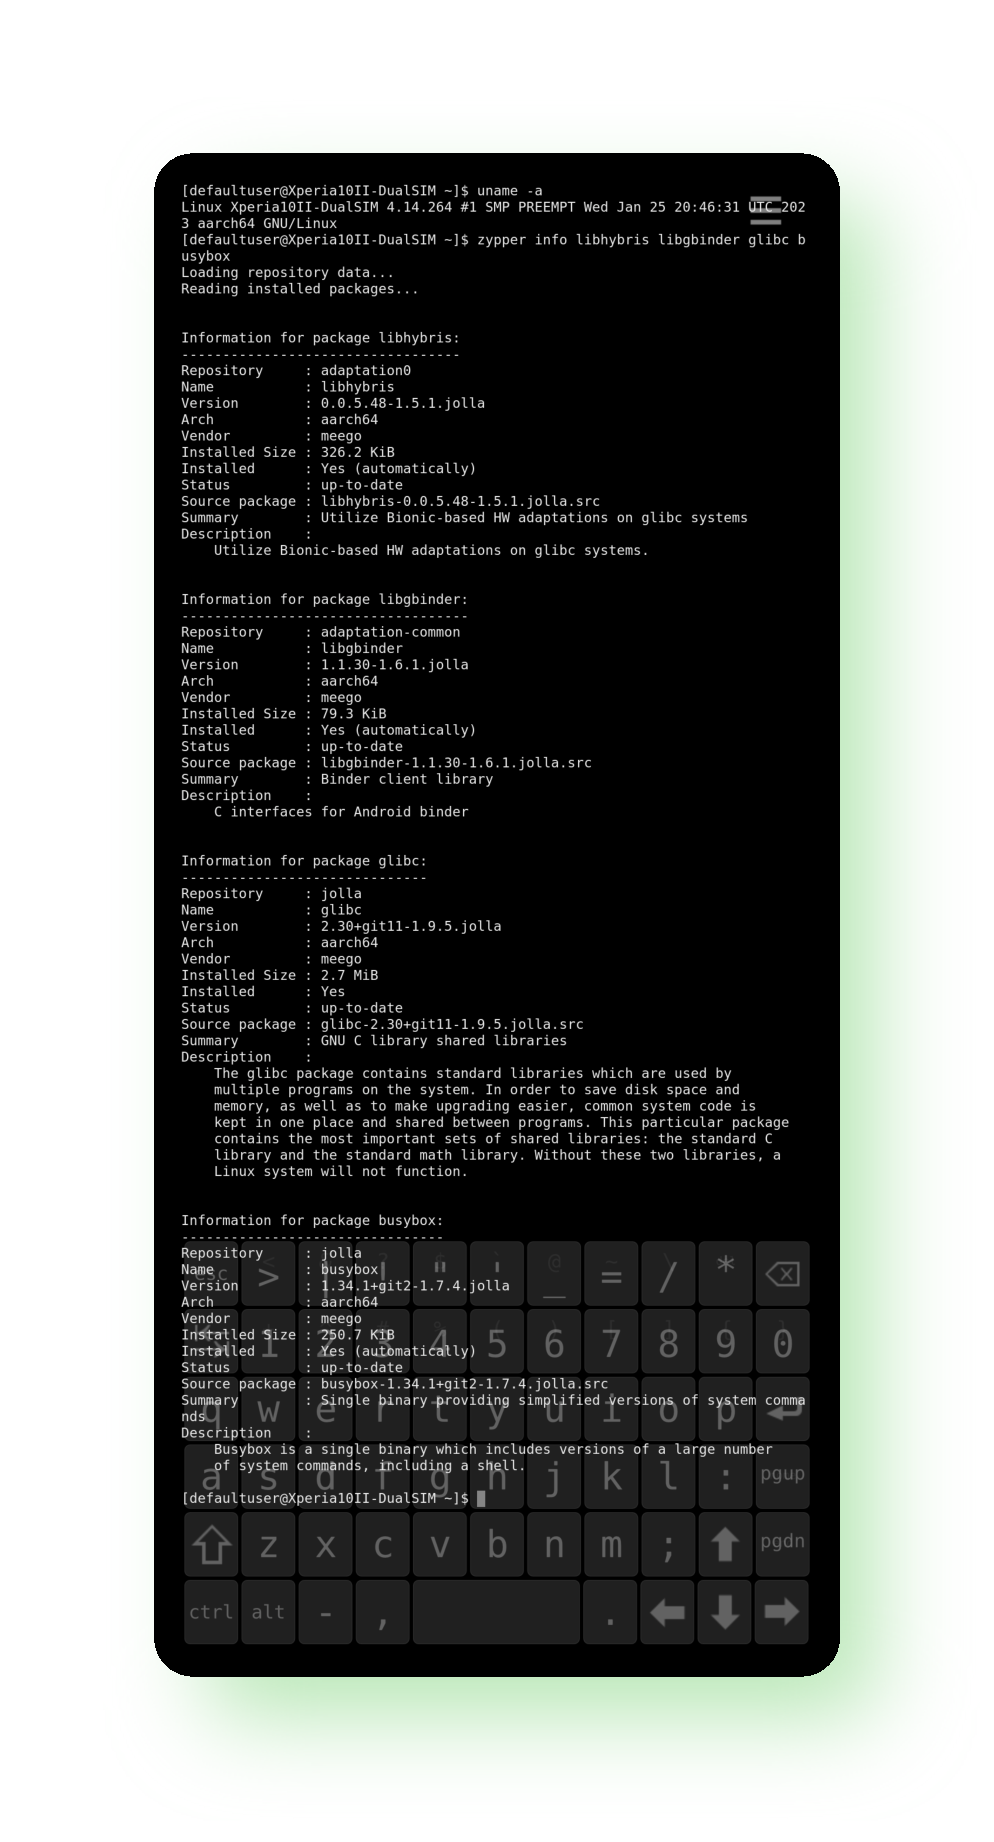
\includegraphics[height=1.0\textheight]{stack-lower}

\end{column}
\end{columns}

\end{frame}
\note{
}

%%%%%%%%%%%%%%%%%%%%%%%%%%%%%%%%%%%%%%%%%

\begin{frame}
\frametitle{Sailfish OS Stack}

\begin{columns}[T]
\begin{column}[T]{0.5\textwidth}
\setlength{\parskip}{0.5em}

\vspace{0.0cm}
\hspace{1.3cm}
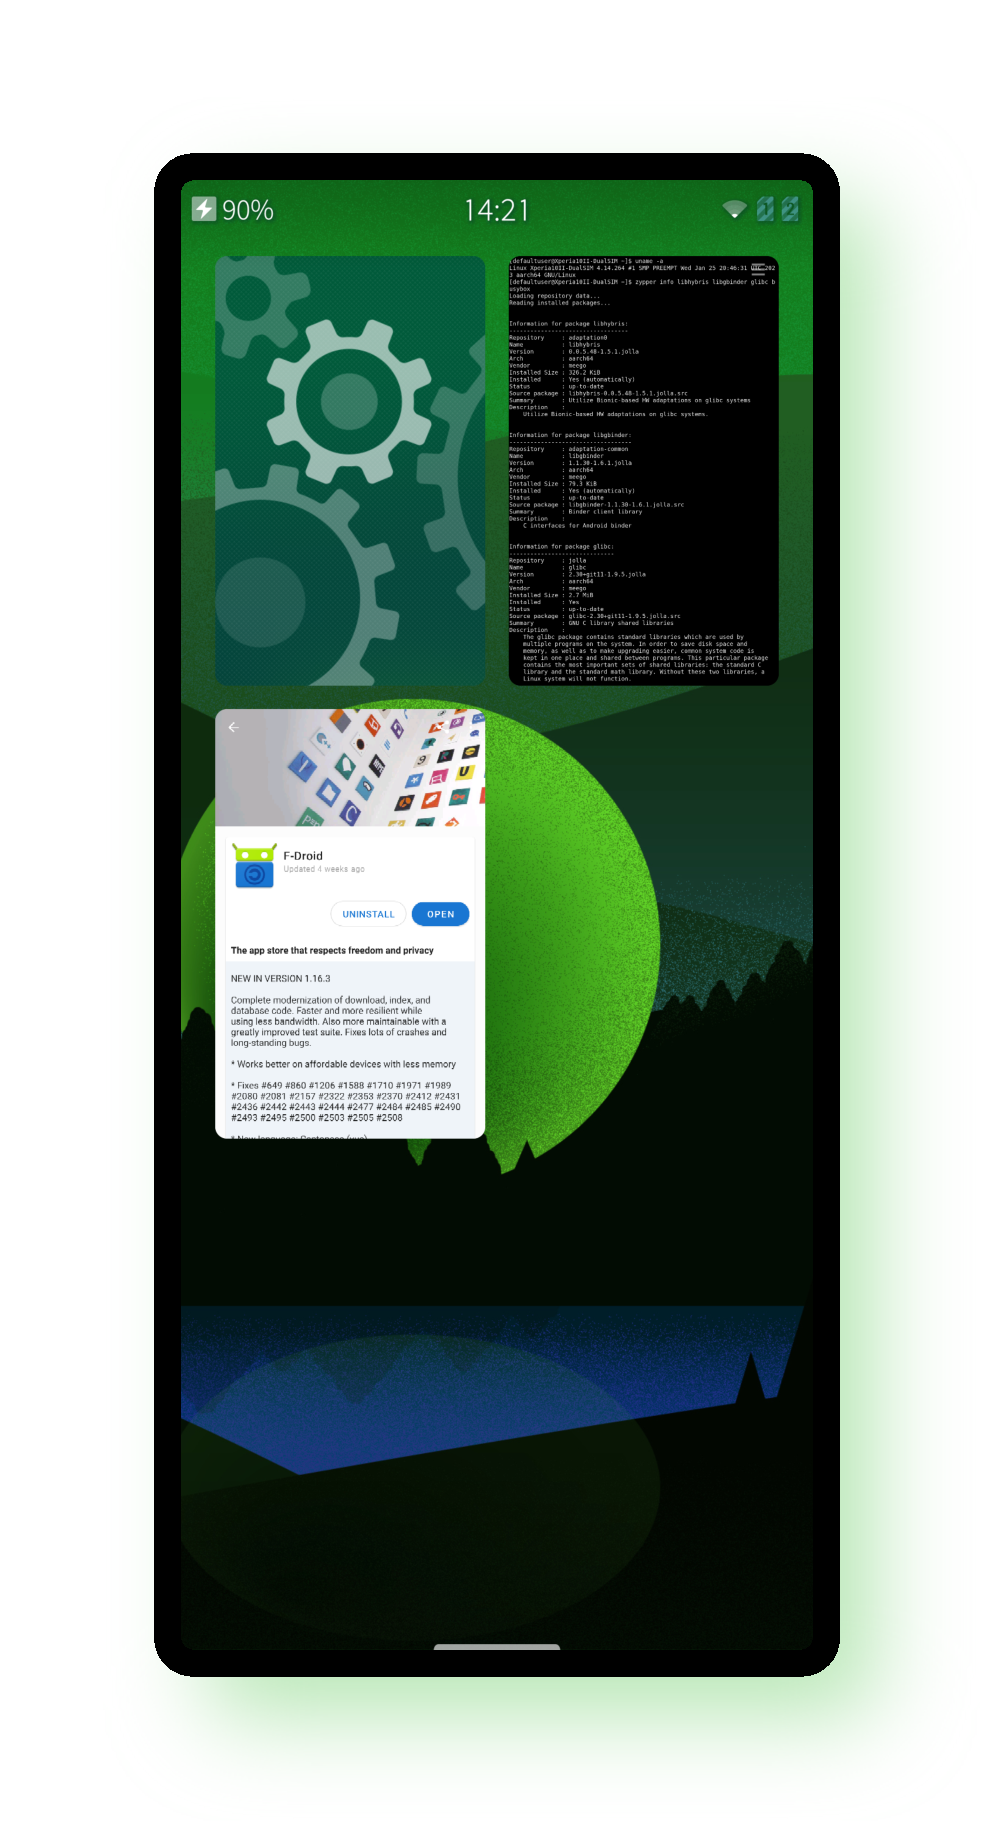
\includegraphics[height=1.0\textheight]{stack-upper}

\end{column}
\begin{column}[T]{0.5\textwidth}
\setlength{\parskip}{0.5em}

\vspace{1.5cm}
\begin{enumerate}
\setcounter{enumi}{6}
\setlength{\parskip}{0.5em}
\item Qt middleware
\item Wayland + Lipstick compositor
\item Silica user interface
\item Lipstick launcher
\item Gecko-based Web browser
\item Android App Support
\end{enumerate}

\end{column}
\end{columns}

\end{frame}
\note{
}

%%%%%%%%%%%%%%%%%%%%%%%%%%%%%%%%%%%%%%%%%

\begin{frame}
\frametitle{Sailfish SDK}

\begin{columns}[T]
\begin{column}[T]{0.5\textwidth}
\setlength{\parskip}{0.5em}

\vspace{0.3cm}
\hspace{0.1cm}
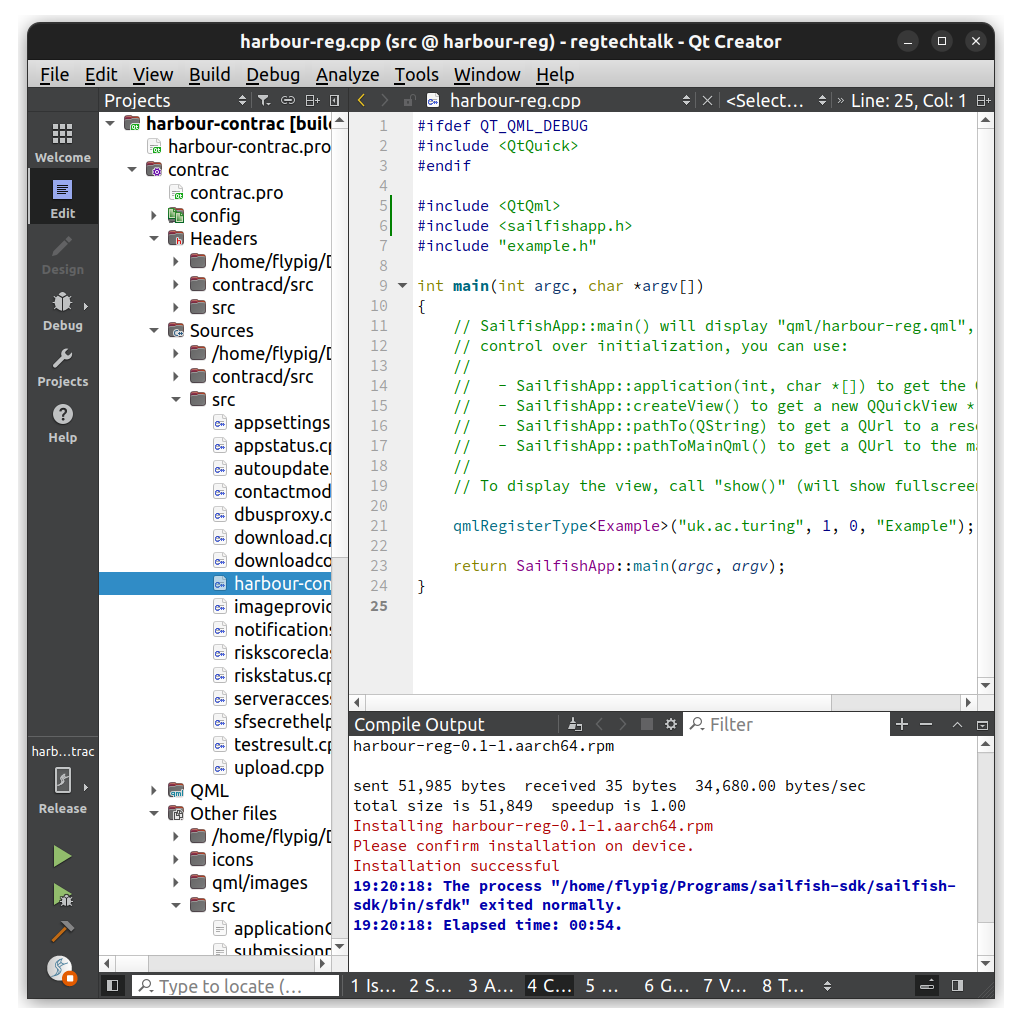
\includegraphics[width=0.9\textwidth]{sailfishide}

\end{column}
\begin{column}[T]{0.5\textwidth}
\setlength{\parskip}{0.5em}

\vspace{0.3cm}
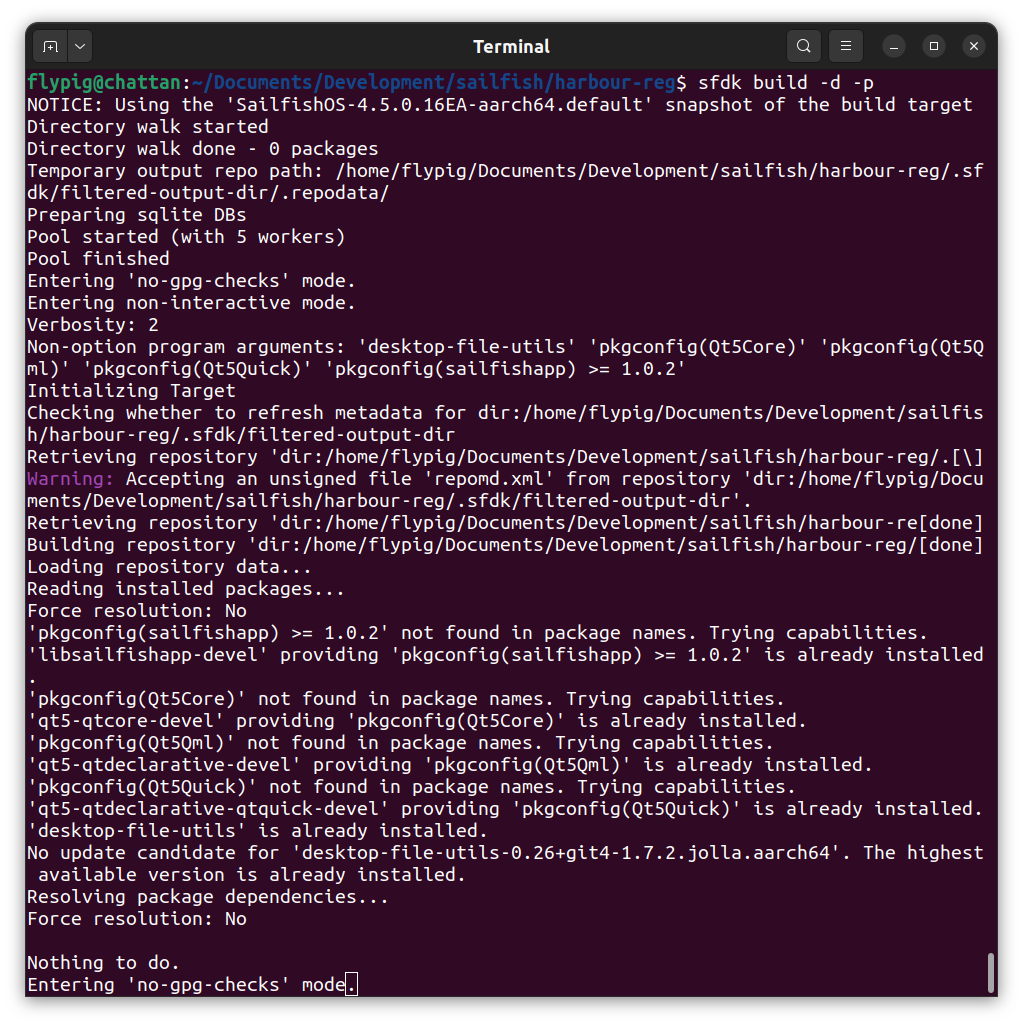
\includegraphics[width=0.9\textwidth]{sfdk}

\end{column}
\end{columns}

\end{frame}
\note{
}

%%%%%%%%%%%%%%%%%%%%%%%%%%%%%%%%%%%%%%%%%

\begin{frame}[fragile]
\frametitle{Further info}
\setlength{\leftmargini}{7.0em}
\vspace{0.8cm}

\begin{itemize}
\setlength{\parskip}{1.0em}
\item[Dev Diary] \, \url{https://www.flypig.co.uk/gecko}
\item[Sailfish Browser] \, \url{https://github.com/sailfishos/sailfish-browser}
\item[gecko-dev] \, \url{https://github.com/llewelld/gecko-dev}
\item[Sailfish OS] \, \url{https://sailfishos.org}
\item[Slides source] \, \url{https://github.com/llewelld/fosdem24-gecko-dev}
\end{itemize}

\end{frame}
\note{
\fontsize{7pt}{8pt}{\bibliographystyle{ieeetr}}
\bibliography{slides}

{\tiny Tux image attribution: lewing@isc.tamu.edu Larry Ewing and The GIMP}
}

%%%%%%%%%%%%%%%%%%%%%%%%%%%%%%%%%%%%%%%%%

\end{document}
